\documentclass{article}
\usepackage{tikz}
\usepackage{mathtools}

\newcommand\then{\rightarrow}
\newcommand\liff{\leftrightarrow}
\newcommand\lxor{\oplus}
\author{Sandra Kohl, Jan Hendrik Kirchner, Max Bernhard Ilsen}

\begin{document}
\section{Exercise \textit{(Multi-Layer Perceptron (8p))}}
\begin{enumerate}
    \item Draw multi-layer perceptron to solve each given logical function
        below.\\
        (We assume a threshold $\Theta$ with $0 < \Theta < 1$ for each neuron.)
        \begin{enumerate}
            \item $x1 \lxor x2$\\
                \begin{center}
                \begin{minipage}{8cm}
                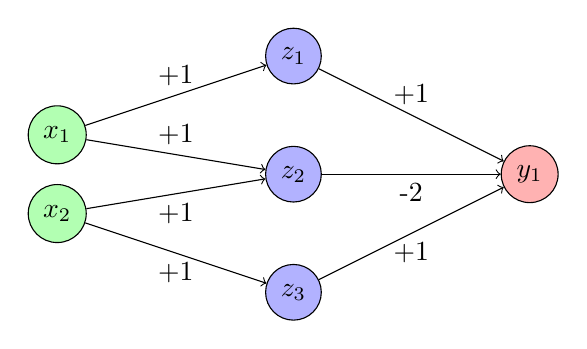
\begin{tikzpicture}
                    \path
                    (0,3) node[circle,draw,fill=green!30](x1) {$x_1$}
                    (0,2) node[circle,draw,fill=green!30](x2) {$x_2$}
                    (3,4) node[circle,draw,fill=blue!30](z1) {$z_1$}
                    (3,2.5) node[circle,draw,fill=blue!30](z2) {$z_2$}
                    (3,1) node[circle,draw,fill=blue!30](z3) {$z_3$}
                    (6,2.5) node[circle,draw,fill=red!30](y1) {$y_1$};

                    \draw[->] (x1) -- node[align=center,above]{+1} (z1);
                    \draw[->] (x1) -- node[align=center,above]{+1} (z2);
                    \draw[->] (x2) -- node[align=center,below]{+1} (z2);
                    \draw[->] (x2) -- node[align=center,below]{+1} (z3);

                    \draw[->] (z1) -- node[align=center,above]{+1} (y1);
                    \draw[->] (z2) -- node[align=center,below]{-2} (y1);
                    \draw[->] (z3) -- node[align=center,below]{+1} (y1);
                \end{tikzpicture}
                \end{minipage}
                \end{center}
            \item $(x_1 \land x_4) \lor (x_2 \land x_3)$\\
                \begin{center}
                \begin{minipage}{8cm}
                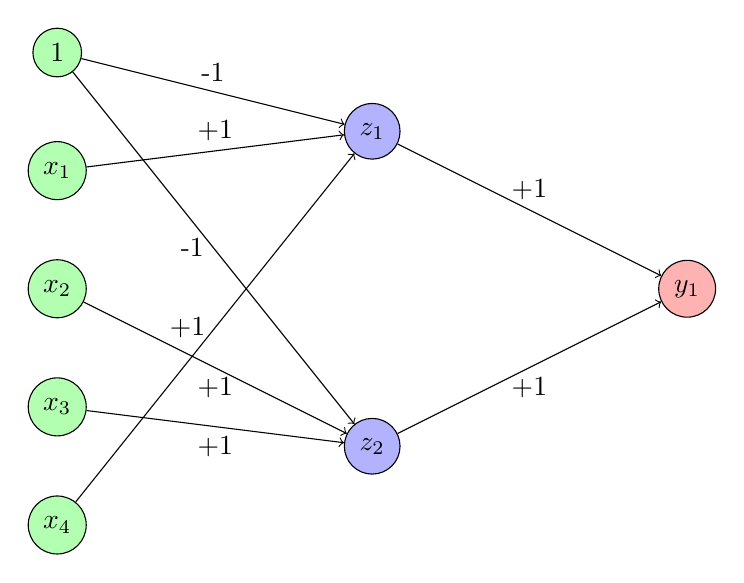
\begin{tikzpicture}
                    \path
                    (0,6) node[circle,draw,fill=green!30](x0) {$1$}
                    (0,4.5) node[circle,draw,fill=green!30](x1) {$x_1$}
                    (0,3) node[circle,draw,fill=green!30](x2) {$x_2$}
                    (0,1.5) node[circle,draw,fill=green!30](x3) {$x_3$}
                    (0,0) node[circle,draw,fill=green!30](x4) {$x_4$}
                    (4,5) node[circle,draw,fill=blue!30](z1) {$z_1$}
                    (4,1) node[circle,draw,fill=blue!30](z2) {$z_2$}
                    (8,3) node[circle,draw,fill=red!30](y1) {$y_1$};

                    \draw[->] (x0) -- node[align=center,above] {-1} (z1);
                    \draw[->] (x0) -- node[align=center,below,left] {-1} (z2);
                    \draw[->] (x1) -- node[align=center,above] {+1} (z1);
                    \draw[->] (x4) -- node[align=center,above,left] {+1} (z1);
                    \draw[->] (x2) -- node[align=center,below] {+1} (z2);
                    \draw[->] (x3) -- node[align=center,below] {+1} (z2);
                    \draw[->] (z1) -- node[align=center,above] {+1} (y1);
                    \draw[->] (z2) -- node[align=center,below] {+1} (y1);
                \end{tikzpicture}
                \end{minipage}
                \end{center}
            \item $x_1 \lor (x_2 \land x_3)$\\
                \begin{center}
                \begin{minipage}{8cm}
                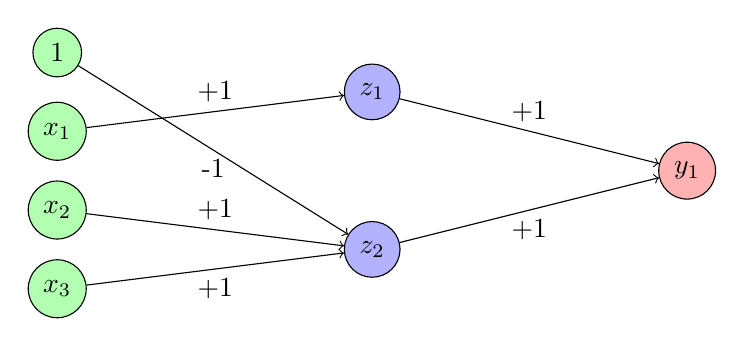
\begin{tikzpicture}
                    \path
                    (0,3) node[circle,draw,fill=green!30](x0) {$1$}
                    (0,2) node[circle,draw,fill=green!30](x1) {$x_1$}
                    (0,1) node[circle,draw,fill=green!30](x2) {$x_2$}
                    (0,0) node[circle,draw,fill=green!30](x3) {$x_3$}
                    (4,2.5) node[circle,draw,fill=blue!30](z1) {$z_1$}
                    (4,0.5) node[circle,draw,fill=blue!30](z2) {$z_2$}
                    (8,1.5) node[circle,draw,fill=red!30](y1) {$y_1$};

                    \draw[->] (x0) -- node[below] {-1} (z2);
                    \draw[->] (x1) -- node[above] {+1} (z1);
                    \draw[->] (x2) -- node[above] {+1} (z2);
                    \draw[->] (x3) -- node[below] {+1} (z2);
                    \draw[->] (z1) -- node[above] {+1} (y1);
                    \draw[->] (z2) -- node[below] {+1} (y1);
                \end{tikzpicture}
                \end{minipage}
                \end{center}
        \end{enumerate}
        \newpage
    \item Calculate the following derivatives:
        \begin{enumerate}
            \item
                \begin{align*}
                    f(x) &= \frac{1}{1+exp(-\lambda x)}  = (1+exp(-\lambda
                    x))^{-1}\\
                    f'(x) &= (-1)*(1+exp(-\lambda x))^{-2}*exp(-\lambda
                    x)*(-\lambda)\\
                    &= \frac{\lambda}{1+exp(-\lambda x)}*\frac{exp(-\lambda
                x)}{1+exp(-\lambda x)}\\
                &= \frac{\lambda}{1+exp(-\lambda x)}*\frac{1+exp(-\lambda
            x)-1}{1+exp(-\lambda x)}\\
            &= \frac{\lambda}{1+exp(-\lambda x)}*(1-\frac{ 1}{1+exp(-\lambda
        x)})\\
        &= \lambda*f(x)*(1-f(x))
    \end{align*}
\item
    \begin{align*}
        f(x) &= \frac{2}{1+exp(-x)} -1  = 2*(1+exp(-x))^{-1}-1\\
        f'(x) &= (-2)*(1+exp(- x))^{-2}*exp(-x)*(-1)-1\\
              &= 2*(1+exp(- x))^{-2}*exp(-x) -1\\
              &= \frac{2}{1+exp(-x)}*\frac{exp(-x)}{1+exp(- x)}-\frac{1+exp(- x)}{1+exp(- x)}\\
              &= \frac{2}{1+exp(-x)}*\frac{exp(-x)-1-exp(- x)}{1+exp(- x)}\\
              &= \frac{2}{1+exp(-x)}*\frac{-1}{1+exp(- x)}\\
              &= \frac{1}{2}(\frac{2}{1+exp(-x)})*(-\frac{2}{1+exp(-x)})\\
              &= \frac{1}{2}(1+\frac{2}{1+exp(-x)} -1)*(1-\frac{2}{1+exp(-x)} -1)\\
              &= \frac{1}{2}(1+f(x))*(1-f(x))
    \end{align*}
        \end{enumerate}
    \item Write down a general sigmoid function and its derivative.
        \begin{align*}
            f(x) &= \frac{|b-a|}{1+exp(-x)}+a  =
            |b-a|*(1+exp(-x))^{-1}+a\\
            f'(x) &= -|b-a|*(1+exp(- x))^{-2}*exp(-x)*(-1)+a\\
                  &= \frac{|b-a|}{1+exp(- x)}*\frac{exp(-x)}{1+exp(- x)}+a\\
                  &= \frac{|b-a|}{1+exp(- x)}*\frac{1+exp(-x)-1}{1+exp(- x)}+a\\
                  &= \frac{|b-a|}{1+exp(- x)}*(\frac{1+exp(-x)}{1+exp(-
        x)}-\frac{1}{1+exp(-x)})+a\\
                  &= \frac{|b-a|}{1+exp(- x)}*(1-\frac{1}{1+exp(-x)})+a\\
                  % &= \frac{|b-a|+a*(1+exp(-x))}{1+exp(- x)}-\frac{1}{1+exp(-x)}\\
                  % &= \frac{|b-a|+a+a*exp(-x)-1}{1+exp(- x)}\\
                  % &= \\
        % ???
        \end{align*}
\end{enumerate}

\section{Exercise \textit{(Backpropagation (4p))}}
\begin{enumerate}
    \item How to avoid local minima in backpropagation?
    \item Explain the generalization and avoiding overfitting.
    \item To prevent overly large weights which cause the high sensitivity of inputs, we apply the
        quadratic regularization term in the error function. Use gradient descent to minimize this
        error function.
\end{enumerate}
\end{document}
